\chapter{Systematic drug repositioning analysis}

\textbf{Key points}
\begin{itemize}
  \item The Functional Therapeutic Chemical Classification System (FTC) provides a descriptor for the function of drugs, which can be used to analyse the systematic relationship between function, structure and indication for approved drugs.
  \item Overall, approved drugs have dissimilar structures and dissimilar functions. When the therapeutic area is considered, the more specific the drug’s indication is, the more similar the structure and function are. These observations are in line with the similar property principle and can be used to isolate drug repositioning hypotheses from the dataset considered.
  \item A drug repositioning hypothesis is a pair of drugs indicated for different therapeutic areas (two ATC levels) but with a high functional similarity value. This method of extraction is called “similarity-based”. I extracted 797 of such pairs and made them openly available through a web application.
  \item The set of repositioning hypotheses can be used to study the relationship between therapeutic areas: some repositioning hypotheses are more frequent between particular therapeutic groups and overlap with known off-label uses.
  \item From the full set of hypotheses, two use-cases are investigated in detail: hypertension and Alzheimer's disease. The drug “similarity-based” repositioning hypotheses are compared against the “toolbox approach”, where FTC categories are directly used as a starting point to forward repurposing opportunities.
  \item Cardiovascular hypertension hypotheses relate mostly to similar pharmacological actions but in different anatomical areas. Alzheimer's disease hypotheses involve biological processes related to the Tau protein and beta-amyloids; the majority of hypotheses find supporting evidence in the biomedical literature.
  \item This analysis concludes the thesis. Chapter 5 sets the work done in the context of the overall drug discovery process and discusses future work and open questions.
\end{itemize}

\textbf{Author's comment}

This chapter is a narrative analysis of the content of the FTC. Results and discussion are mixed together as I believe it makes the text more understandable and clarifies the reasoning behind the work. A methods section is provided at the end, describing the details of the analyses performed if needed.

\hrulefill

\section{Introduction}
I decided to look at drug repositioning from the perspective of the mode and mechanism of action (Chapter 1). The implementation of a solution required first some theoretical basis to be set, namely the black box model of the cell, specified using description logics (Chapter 2). The FTC then implemented the theory, as presented in the previous chapter (Chapter 3), and was evaluated against existing solutions to assess the relevance of the approach. This coming chapter will present the biological analysis performed over the content of FTC, in order to more directly address drug repositioning concerns.

As the FTC characterises the concept of function in a systematic fashion, the obvious questions to ask are: How does it relates to the chemical structure? Do similar compounds have similar functions? What about the indication? Is there any relation between function, structure and therapeutic usage?

In this regard, the analysis below first identifies the repositioning hypotheses present in the FTC and discusses the relevance of function in the process. Secondly, the extracted hypotheses are examined in depth and interpreted from a biological viewpoint. Because the FTC provides systemic insight on the drug repositioning topic, it is therefore possible to explore the broad relationship between therapeutic areas as well as the connection between drug repositioning and off-label uses. Finally, a couple of detailed use-cases are discussed: cardiovascular hypertension and Alzheimer's disease. These pathologies will serve to demonstrate how two different methodologies can be applied over the FTC to extract hypotheses:  the “similarity-based” and the “toolbox” approaches.

This chapter is more focused on the biology and its interpretation. The content of FTC is dissected using semantic similarity and mode of action (MoA) cherry-picking. The conclusions drawn in this chapter will introduce future work to be done, as well as new leads to be explored.

\section{Structure, function and indication of drugs}
The most commonly accepted rule in drug discovery is probably the similar property principle: Similar structures have similar biological activities - or functions \citep{martin2002structurally} \citep{kubinyi1998similarity} \citep{johnson1990concepts}. Despite being true in some cases, there are plenty of examples in contradiction with this rule. As the FTC provides a unique characterisation of the function of chemical compounds, I decided to analyse the structure/function relationship for approved drugs, with a systematic stance. Before being able to do so, it is however necessary to choose adequate descriptors; the function will be represented by the FTC, but the structural descriptor still remains to be selected. This preliminary characterisation will allow me to then compare each drug’s chemical structure against function in a systematic fashion and derive repositioning hypotheses.

\subsection{Structural descriptor selection}
The structure of two chemical compounds can be compared in a variety of ways, depending on the application \citep{johnson1990concepts}. In my case, the main motivation was to find a representative descriptor with a good dynamic range for the dataset considered - a thousand approved drugs. Moreover, the structural descriptor must be relatively easy to handle, fast to compute and with an explicit meaning, solely depending on the molecule and not on external factors.

In order to match these requirements, I decided to focus only on two-dimensional chemical structures, as numerous methods exist to compute them and because they are more accurate for predicting target affinity than three-dimensional descriptors \citep{nettles2006bridging}, and therefore more suited to study bioactivity. The interpretation of the results is also easier and directly related to the chemical groups present in the structure \citep{todeschini2009molecular}.

Two-dimensional structures can be represented by fingerprinting methods (//ref see material and methods). Numerous implementations exist, varying in the chemical patterns encoded. I chose to try four of them over my dataset: hybridization, extended, MACCS and PubChem fingerprints (//ref see details in method). These methods were selected because they are readily available in the Chemistry Development Kit (//cite - CDK) and relatively different one from another, therefore providing independent yet comparable results. Figure \ref{fig4-1} illustrates this: The plot shows the density distribution of similarity values between pairs of drugs for the various fingerprinting methods considered (//ref method).

\begin{figure}[H]
    \centering
    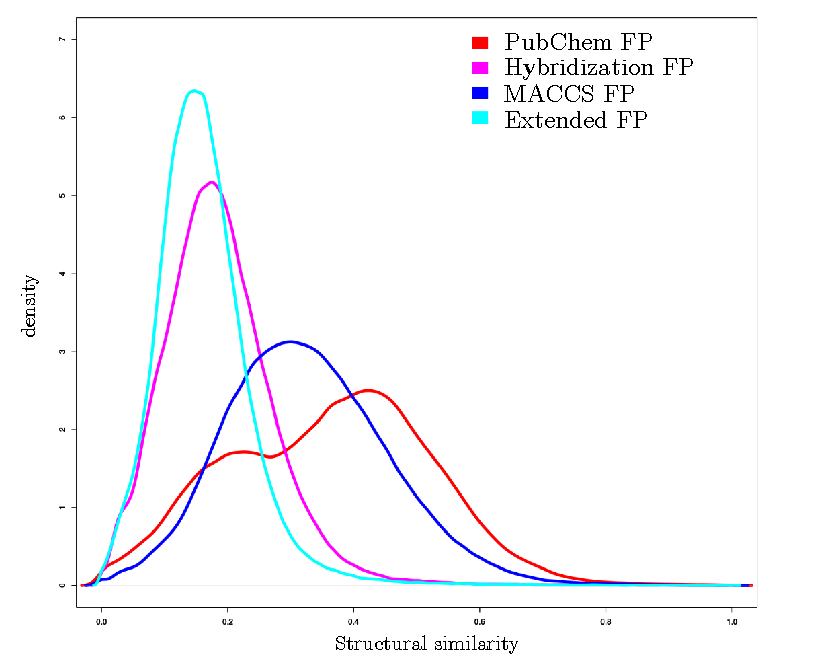
\includegraphics{fig4-1}
    \caption{Kernel density distribution for various chemical fingerprinting (FP) methods. All the methods have been applied as implemented in the CDK (cf material and methods). Each approved drug was compared against all other approved drugs (pairwise comparison), in order to determine which methodology provides the most suitable distribution to study the dataset.}
    \label{fig4-1}
\end{figure}

Different methods have different curves: MACCS and PubChem fingerprinting functions have wider distributions, as shown by the value of the interquartile range, higher than with the other methods (Table \ref{fpmethods}). The distribution of structural similarity values is an important criterion for this analysis, as it reflects the spread of the data. In my case, the wider, the more dynamic and therefore the better.

\begin{center}
\small
    \begin{tabular}{| l | l | l | l | l | l || l | l | l | l |}
    \hline
 & PubChem & Hybrid. & MACCS & Ext. & Mean corr. & Qu.1 & Mean & Qu.3 & Range \\ \hline \hline 
PubChem & X & 0.65 & 0.61 & 0.73 & 0.66 & 0.24 & 0.36 & 0.47 & 0.24 \\ \hline
Hybrid. & 0.65 & X & 0.66 & 0.84 & 0.72 & 0.13 & 0.19 & 0.24 & 0.11 \\ \hline
MACCS & 0.61 & 0.66 & X & 0.65 & 0.64 & 0.24 & 0.33 & 0.41 & 0.17 \\ \hline
MACCS & 0.61 & 0.66 & X & 0.65 & 0.64 & 0.24 & 0.33 & 0.41 & 0.17 \\ \hline
Ext. & 0.73 & 0.84 & 0.65 & X & 0.74 & 0.11 & 0.16 & 0.2 & 0.09 \\ \hline
    \end{tabular} \captionof{table}{Correlation values between various fingerprinting methodologies. "Mean corr." stands for the mean value of the correlation coefficients. "Ext." stand for Extended fingerprinter, "Hybrid." for Hybridization. "Range" describes the interquartile range (Qu.3 - Qu.1)}
    \label{fpmethods}
\end{center}

Nonetheless, the agreement between the various fingerprinting methodologies also has to be considered: The goal is to find an average structural descriptor, somehow representative and not too polarised, in order to derive systematic conclusions later on. The agreement between methodologies was defined by the Pearson correlation coefficient (//ref see methods) and is presented on table XXX. Briefly, this coefficient ranges between -1 to 1 and reflects how correlated two series of points are, 1 being a total positive correlation and -1 a total negative correlation. As each method is compared against all other fingerprinting methodologies, I considered the average of Pearson’s coefficients as a representative metric; the higher the value, the more a method agrees with the others. From this heuristic, table \ref{fpmethods} shows that the extended fingerprinting method is the most in line with the others (mean = 0.74), MACCS being the one agreeing the least (mean = 0.64). Nonetheless, all methods have pretty similar average values (see Table \ref{fpmethods}), meaning that all techniques reach overall the same level of agreement. Note that the extended and hybridisation fingerprints have the highest agreement value between them (0.84), reflecting the closeness in the implementation (personal discussion with CDK developers).

Based on these results, I decided to use the PubChem fingerprint to represent the chemical structure of drugs. The method distributes best the dataset analysed and agrees well with the other fingerprinting methodologies tested, features required for the subsequent drug repositioning analysis.

\subsection{Dissimilar structures have dissimilar functions}
The functional descriptor derives from the structure of the FTC and the semantic similarity. Given a pair of drugs, the closer they are present in the taxonomic tree, the more similar they are inferred to be (//ref section ch2 and material and method). From this selection of the functional and structural descriptors, it is possible to study the relationship between drugs.

The similar property principle states that similar structures have similar biological activities. The rule was derived from QSAR analyses, where the goal is to try to fit a chemical structure inside a cavity, for instance the active site of an enzyme (//cite “Molecular Descriptors for Chemoinformatics”). In such a case, the rule is intuitively acceptable, yet numerous exceptions are known. The functional descriptor introduced can abstract away from this physical viewpoint and appreciate the similarity relationship in a systematic fashion. In this regard, Figure 4-2 illustrates the distribution of similarity values for all pairs of drugs. Note that the indication is not taken into consideration at this stage.

\begin{figure}[H]
    \centering
    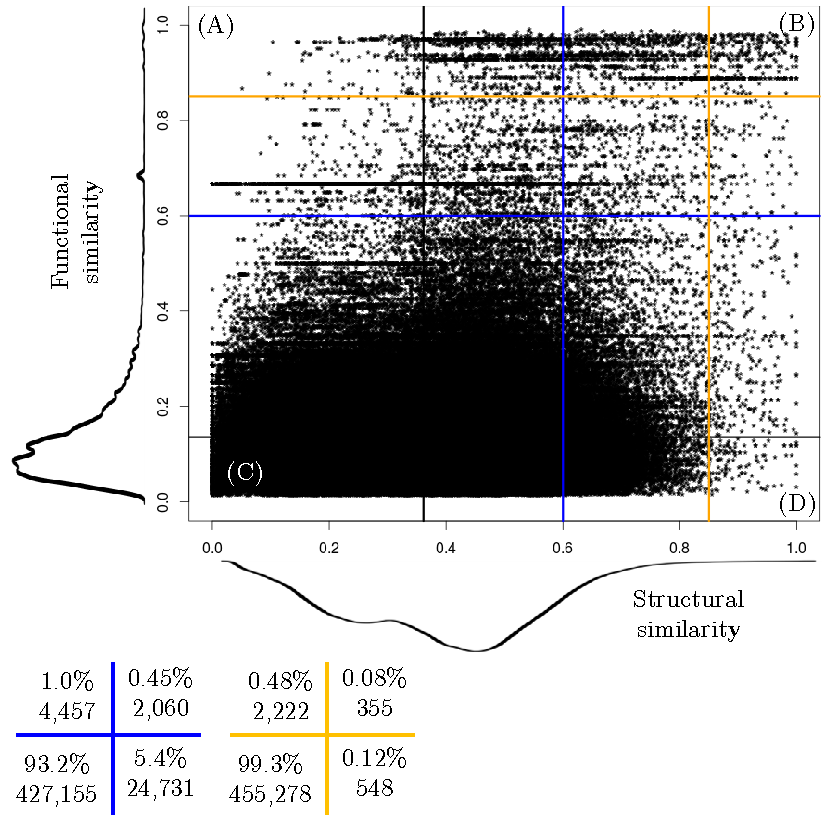
\includegraphics{fig4-2}
    \caption{Functional against structural similarity values for approved drugs. Each drug is compared against all other drugs (pairwise comparison) using both the structural and functional descriptors and corresponding to one dot or data point on the graph. Two different arbitrary thresholds are applied, represented by the blue and orange lines on the graph. The blue line separates the fairly similar values (\textgreater 0.6) from the rest, and the orange ones split up the highly similar (\textgreater 0.85) from the rest of the dataset. The graph is divided and labelled into 4 sections, identified by letters on the figure. The numbers of data points present in each one of these areas are listed on the table below the plot. The kernel density distribution are plotted on the side of the axis (qualitative) in order to appreciate the distribution of the data.}
    \label{fig4-2}
\end{figure}

The scatterplot is further divided into areas, broadly separating groups of drugs based on their relative similarity. I chose to consider two different thresholds, in order to separate the similar compounds from the dissimilar ones, represented by the blue and orange lines in Figure \ref{fig4-2}. The first threshold (blue) is set at an arbitrary similarity value of 0.6. This number appears able to separate the relatively similar from dissimilar compounds, and is derived from observations made in Figure 4-9 (discussed later). The second threshold (orange line) was set at the arbitrary value of 0.85; it separates strongly similar compounds from the rest. This value is generally accepted as a cut-off (\cite{chemsimwiki} and personal discussions). The two thresholds reveal the same trend of data distribution (Table \ref{fpmethods} and Figure \ref{fig4-2}) in their different areas.

From the distribution of values on the graph, it is clear that the large majority of molecules have dissimilar structures and dissimilar functions. This corresponds to area C on the graph \ref{fig4-2}, containing either 93\% or up to 99\% of the data points, depending on the threshold considered. This result can be explained as follows: approved drugs cover a wide range of different bioactivities (dissimilar functions), affecting numerous distinct processes involved in diseases. Their pharmacology is mediated via an interaction with different protein targets, therefore different chemical structures are needed. Moreover, for patent concerns, dissimilar structures are usually sought in order to maximise intellectual protection \citep{barratt2012drug}. This explanation is consistent with the low number of drugs with similar functions and similar structures (area B on the graph), pairs in agreement with the similar property principle.

Interestingly, a number of drugs are not in line with the similarity rule, represented by the data points in areas A and D. Such pairs have either similar functions with low structural resemblance (area A) or high structural similarities with little shared bioactivity (area D). This observation shows the challenge in drug discovery to relate function and structure: similar MoAs can be obtained with different structures (area A), and just because two structures are similar does not imply that they will trigger the same biological effect (area D).

Two conclusions can be derived from this plot. First, the graph reveals that most drugs have dissimilar structures and dissimilar functions, which I interpret as complementary and in line with the similar property principle. The relation between these pairs of compounds is not informative for drug repositioning and they can later be filtered out. Secondly, the plot enables the identification of exceptions to the similarity rule (areas A and D). These pairs of drugs are of particular interest, as they represent an unexpected pharmacology, not in line with the rule and therefore more difficult to identify. Such pairs are present in limited quantities, yet they intriguingly more numerous than the pairs respecting the principle and will be investigated in more detail.

So far structure has only been compared to function; yet in order to be more meaningful, the indication of the drugs also has to be considered in the analysis. Intuitively, compounds present in the same therapeutic group should share higher similarity values, reflecting that they target related proteins and have more similar functions.

\subsection{The more specific an indication is, the more similar the function and structure are}
The ultimate value of a chemical compound arises from its therapeutic usage. In this regard, the legal indication of a drug is the gold-standard of information. This section further analyses the functional and structural descriptors introduced before and compares them against the legal indication and usage, as represented in the Anatomical Therapeutic Chemical Classification System (ATC). The goal of this comparison is to see whether the descriptors can further provide any meaningful information regarding the indication of a drug, which could be used to retrieve repositioning hypotheses.

According to the similar property principle, drugs present in the same therapeutic group should have on average relatively closer structures and functions. In order to validate this assumption, I considered the five hierarchical levels of the ATC as a representation of the specificity of the indication, with the first or top level of the ATC representing generic and broadly defined indications and the fourth level or bottom level characterising very precisely the indication of a compound (see Figure \ref{fig4-3}).

\begin{figure}[H]
    \centering
    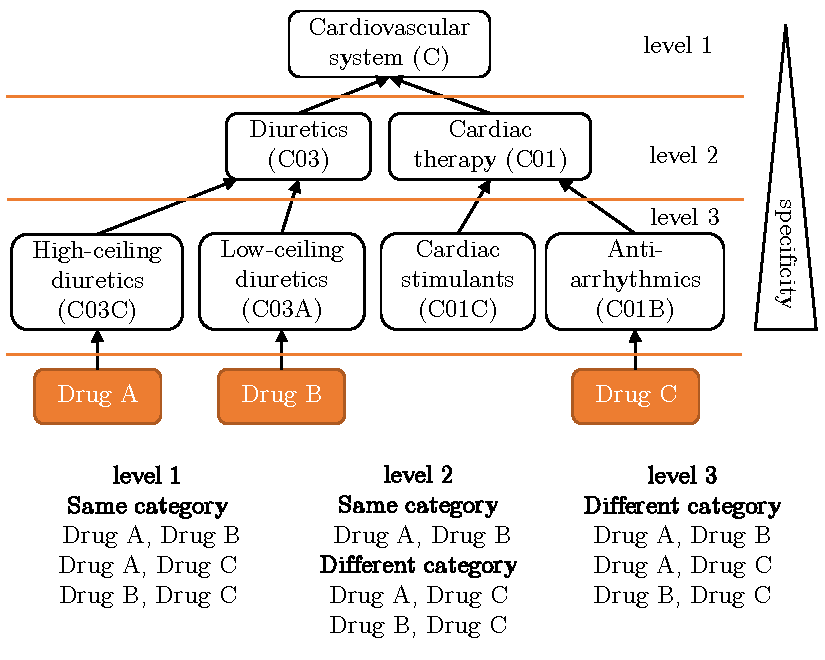
\includegraphics{fig4-3}
    \caption{Specificity of the indication of a drug as represented in the ATC. The ATC captures drug’s indication and is organised over 5 levels (only 4 shown here for clarity), 1 being the highest and most generic level. When descending the tree, the specificity of the indication or action increases. Pairs of drugs can be flagged as belonging to either the same or different ATC category, depending on the level considered (resolution). Three examples are given on the figure in this regards, for the drugs A, B and C. For instance, when only the level 1 is considered, all pairs of drugs are present in the same category (“Cardiovascular system”). When the level 2 is considered, the pair of drugs A and B still belong to the same category (“Diuretics”), but these two drugs are not sharing the indication of drug 3, “Cardiac therapy”. At a resolution of the level 3, each drug has a separate indication/action.}
    \label{fig4-3}
\end{figure}

It is possible to use this definition of the specificity of an indication to filter pairs of drugs and look at the overall evolution of structural and functional similarities. Such an analysis is shown in Figure 4-4, where only pairs of drugs sharing a common indication are shown. When the specificity of the indication increases, represented by the increasing number of the ATC level considered, the average functional and structural similarity increases too.

\begin{figure}[H]
    \centering
    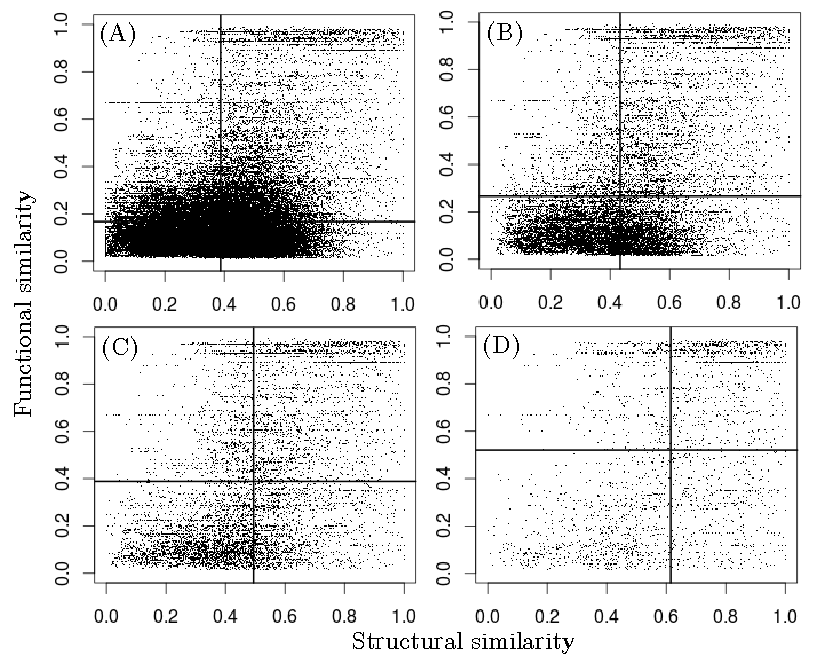
\includegraphics{fig4-4}
    \caption{Distribution of the functional and structural similarity values for pairs of drugs present in the same ATC categories (same indication). The different panels reflect the increasing specificity of the indication of the drugs. X axes is the structural similarity and Y axes is the functional similarity (calculated as with previous graphs). (A) 1 ATC level resolution. (B) 2 ATC level resolution. (C) 3 ATC level resolution. (D) 4 ATC level resolution. Conceptual explanation of resolution and levels is available on figure \ref{fig4-3}. When the specificity of the indication increases (resolution increasing), the average functional and structural similarity values increases too (black lines).}
    \label{fig4-4}
\end{figure}

On the contrary, when only pairs of drugs indicated for increasingly different indications are compared, the average similarity stays the same, as shown on Figure \ref{fig4-5} and summarised Table \ref{tablespecind}.

\begin{figure}[ht]
    \centering
    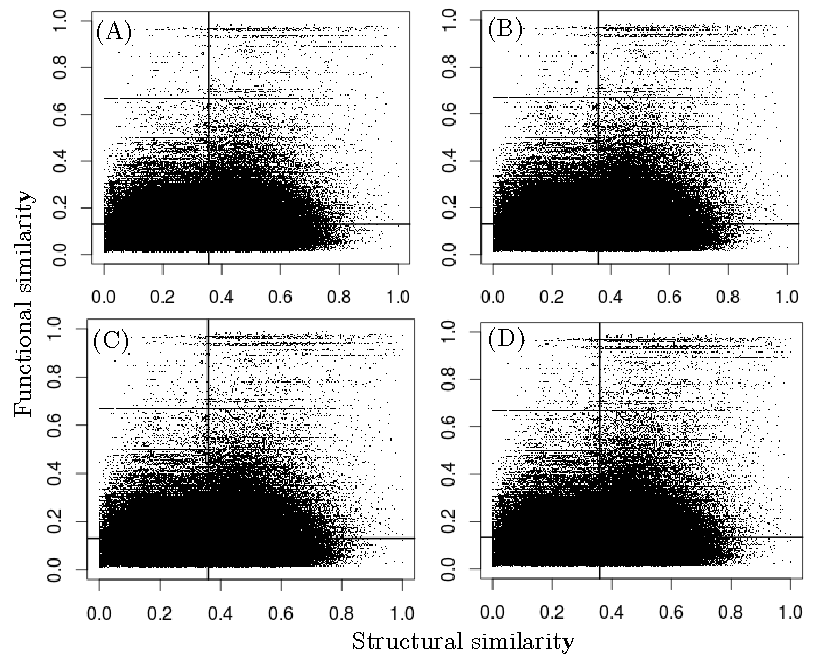
\includegraphics{fig4-5}
    \caption{Distribution of the functional and structural similarity values for pairs of drugs present in the same ATC categories (same indication). The different panels reflect the increasing specificity of the indication of the drugs. X axes is the structural similarity and Y axes is the functional similarity (calculated as with previous graphs). (A) 1 ATC level resolution. (B) 2 ATC level resolution. (C) 3 ATC level resolution. (D) 4 ATC level resolution. Conceptual explanation of resolution and levels is available on Figure 4-3. When the specificity of the indication increases (resolution increasing), the average functional and structural similarity values increases too (black lines).}
    \label{fig4-5}
\end{figure}

Figures 4-6 and 4-7 respectively show the kernel densities of the structural and functional similarities values for the pairs of drugs sharing an indication at a given ATC level. Note that the two descriptors have different behaviours. The structural similarity appears centred in the middle of the graph, and slowly evolves towards higher similarity values with indication specificity. A jump is observed from level 3 to 4 (brown curve on plot 4-6), and is manifested by a larger increase in the average value. This observation is explained by the very definition of the indication coming from the ATC: level 4 handles the categorisation of drugs based on their chemical structures (cf fig definition ATC - ch3 //ref), therefore it is more likely for a pair of molecules present in the same fourth level ATC category to have very similar structures.

\begin{center}
\small
    \begin{tabular}{| l | l | l | l | l | l |}
    \hline
 & Specificity of indication (ATC level) & 1 & 2 & 3 & 4 \\ \hline \hline
Same indication & Structure similarity & 0.39 & 0.43 & 0.49 & 0.62 \\ 
 & Function similarity & 0.17 & 0.27 & 0.39 & 0.52 \\ \hline
Different indication & Structure similarity & 0.36 & 0.36 & 0.36 & 0.36 \\
 & Function similarity & 0.13 & 0.13 & 0.13 & 0.13 \\ \hline
    \end{tabular} \captionof{table}{Evolution of the specificity of indication with the ATC levels. Increasingly similar indications have increasingly similar functional and structural values. The functional and structural similarity values are not evolving when increasingly different indications are considered.}
    \label{tablespecind}
\end{center}

\begin{figure}[H]
    \centering
    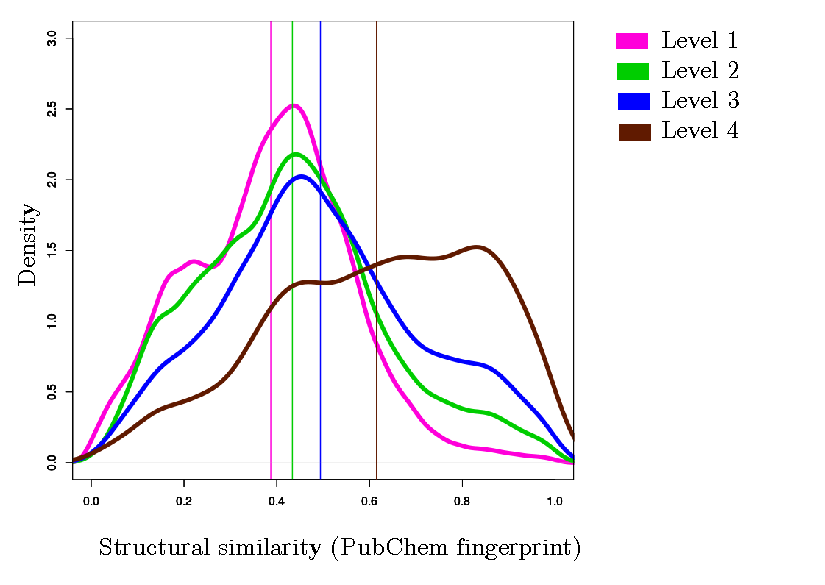
\includegraphics{fig4-6}
    \caption{Kernel density distribution of the structural similarity values for drugs sharing an indication. All ATC categories have been considered. Each curve represent an ATC resolution level, as indicated on the legend. Conceptual explanation of resolution levels is available on Figure \ref{fig4-3}. Solid vertical lines are the corresponding means. This graph shows that with an increasingly specific indication (increasing resolution) the average structural similarity values increase too.}
    \label{fig4-6}
\end{figure}

The functional similarities steadily increase on average (see table with averages). With this descriptor, the relative changes in similarities between different ATC levels are more located on the extremes, as shown in figure \ref{fig4-7}: when the specificity of the indication increases, the number of low similarity values decreases, giving relatively more weight to the high ones.

\begin{figure}[H]
    \centering
    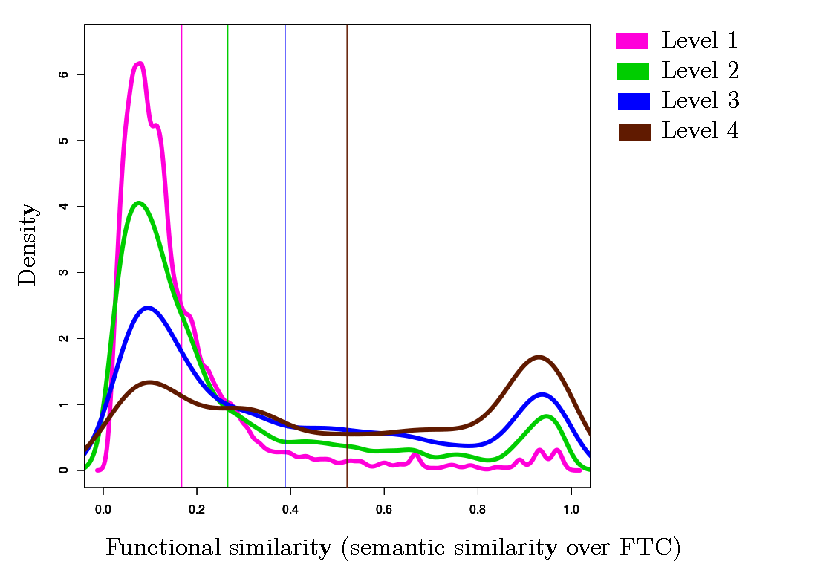
\includegraphics{fig4-7}
    \caption{Kernel density distribution of the functional similarity values for drugs sharing an indication. All ATC categories have been considered. Each curve represent an ATC resolution level, as indicated on the legend. Conceptual explanation of resolution levels is available on Figure \ref{fig4-3}. Solid vertical lines are the corresponding means. This graph shows that with an increasingly specific indication (increasing resolution) the average functional similarity values increase too.}
    \label{fig4-7}
\end{figure}

Taken together, these results confirm the similarity principle at a systematic scale: on average, drugs with closely related indications are structurally and functionally similar, as captured by the descriptors used. As an example, the plot showed in Figure 4-4 panel D displays the highest average similarity, when the indication is the most specific (highest ATC level). This average similarity value was used to set the threshold level at 0.6 in Figure \ref{fig4-2}; it separates functionally similar compounds from the rest. Interestingly, on the same graph (Figure \ref{fig4-4}-D), some of the pairs still have low similarity values (structural and functional lower than 0.3); these points are outliers to the similar property principle and reflect the limits of the descriptors. I performed an error analysis in order to identify the reasons behind the non-respect of the rule by these drugs. The pair of drugs dipyridamole and epoprostenol is a good illustration of the most common cases of misclassification. These two drugs have a relative functional similarity of 0.10 and a structural similarity of 0.14, despite being both categorised as “Platelet aggregation inhibitors” in the ATC (code: B01AC). Although resulting in the same biological outcome and clinical usage, these two drugs are mainly targeting different proteins, a phosphodiesterase in the case of dipyridamole and the P2Y purinoceptor 12 in the case of epoprostenol. In order to interact with these receptors, two different chemical structures are needed and it is therefore expected that the two molecules would have different structures (see Figure 4-8). However, the MoAs from the FTC are not shared either, which comes from missing annotations on the protein targets or because the molecular root of the effect is unknown. It is therefore also not possible to relate these two drugs based on their functions, because of lack of recorded knowledge.

\begin{figure}[H]
    \centering
    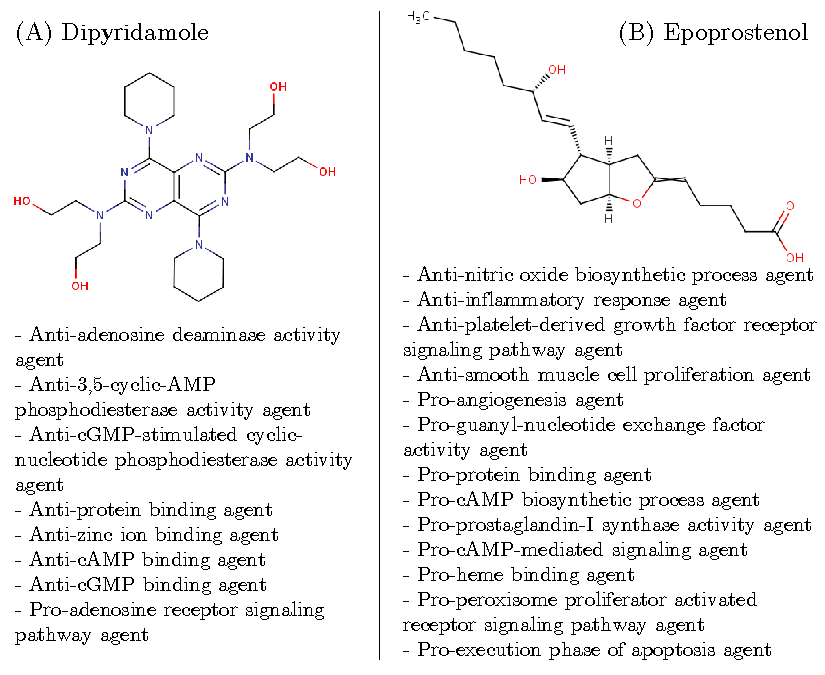
\includegraphics{fig4-8}
    \caption{Example of pair of drugs with low structural and functional similarity values, yet classified in the same ATC category and used for the same clinical indication (“platelet aggregation inhibitors”). (A) Chemical structure and list of FTC categories inside which the dipyridamole was classified. (B) Molecular structure and list of FTC categories inside which the epoprostenol molecule was classified. These two drugs do not share any of the FTC categories listed (functional similarity = 0.10) and their molecular structures are dissimilar (structural similarity = 0.14).}
    \label{fig4-8}
\end{figure}

The figures presented in this section show an observation of primary importance for drug repositioning: the computational descriptors used are able to serve as a proxy for the expected behaviour of the concepts of function and structure in regards to the real clinical indication of a drug. The more similar a pair of drugs are based on either their functional or structural features, the more likely these drugs are clinically indicated for the same sets of diseases.

Note that the data analysis shown in the two previous sections only identified average patterns; particular data points were not taken into considerations. Some exceptions or outliers exists, which will be considered as starting points to formulate drug repositioning hypotheses.

\subsection{The more specific an indication is, the more similar the function and structure are}
//TODO
